\subsection{Initialization}
\label{sec:genetic_programming:initialization}
  As with other evolutionary algorithms, the algorithm starts by generating a
  population of random individuals.
  
  There are many ways to generate random individuals, but a very common (and
  simple) method is the \emph{grow 
  method}~\autocite{kozaGeneticProgrammingProgramming1992a}.
  In this method, a maximum height is defined, and the algorithm then creates a
  random tree with a given minimum height and a maximum height.

  \begin{remark}
    A tree with a height of 0 is a tree with only one node, the root.
  \end{remark}

  The grow method then proceeds to recursively generate the trees with random
  nodes until a terminal node is selected or the maximum height is reached.
  This method is shown in \vref{lst:bg:gp:grow}.

  \begin{code}{
    The grow method for generating random trees.
  }{
    label=lst:bg:gp:grow
  }{kotlin}
    // Given:
    val lo: ~$\mathbb{N}$~ // Minimum height
    val hi: ~$\mathbb{N}$~ // Maximum height
    require(lo ~$\leq$~ hi)
    val n = random.int(lo..hi) // Random height
    fun grow(ts: Set<Terminal>, fs: Set<Function>, depth: ~$\mathbb{N}$~) {
      require(ts != ~$\emptyset$~ && fs != ~$\emptyset$~)
      val c = ~$\emptyset$~
      if (
        depth == n || (depth ~$\geq$~ lo && random.double(0..1) ~$\leq$~ ts.size / (ts.size + fs.size))
      ) {
      // $d = n \lor \left(d \geq l \land \mathrm{random}() < \mathlarger{\frac{|\mathcal{T}|}{|\mathcal{T}| + |\mathcal{F}|}}\right)$
        return random node from ts
      } else {
        val f = random node from fs
        for (i in 1..arity(f)) {
          c += grow(ts, fs, d + 1)
        }
        return a tree with f as root and c as children
      }
    }
  \end{code}

  With this method, the algorithm can generate trees where the size of the 
  longest path from the root to a leaf is a number \(n \in [l, h]\).

  Now that the algorithm can generate random trees, it can generate a random
  population of trees by generating a random tree for each individual in the
  population.
  Assuming a population size of \(p = 4\), a maximum height of \(h = 3\), a
  minimum height of \(l = 1\), and the primitives set defined in the previous
  section, the algorithm could generate the population: 
  \(
    \mathbf{P} = \{\mathbf{I}_1,\,\mathbf{I}_2,\,\mathbf{I}_3,\,\mathbf{I}_4\} 
      = \left\{
        \frac{3}{\sin(2)} \times 5^3,\,
        7 - (5 + \sin(x)),\,
        7 + 2,\,
        5x^2
      \right\}
  \), as shown in \vref{fig:genetic_programming:initialization:population}.

  \begin{figure}[ht!]
    \centering
    \begin{subfigure}[t]{0.4\textwidth}
      \centering
      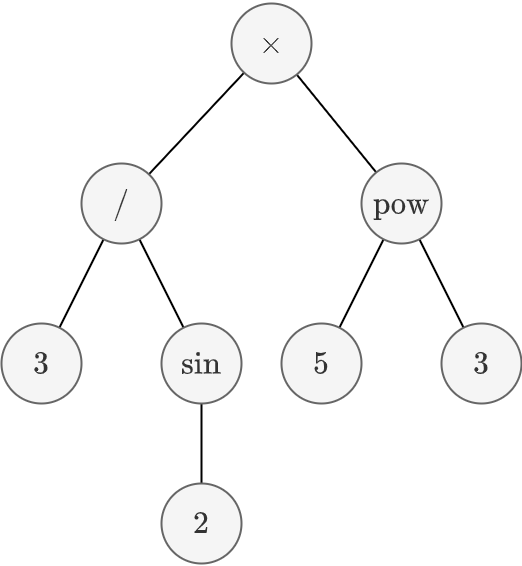
\includegraphics[height=5.5cm]{img/theoretical_framework/GP Initial Population 1.png}
      \caption{\(\mathbf{I}_1 = \mathlarger{\frac{3}{\sin(2)}} \times 5^3\)}
      \label{fig:genetic_programming:initialization:population:1}
    \end{subfigure}
    \begin{subfigure}[t]{0.4\textwidth}
      \centering
      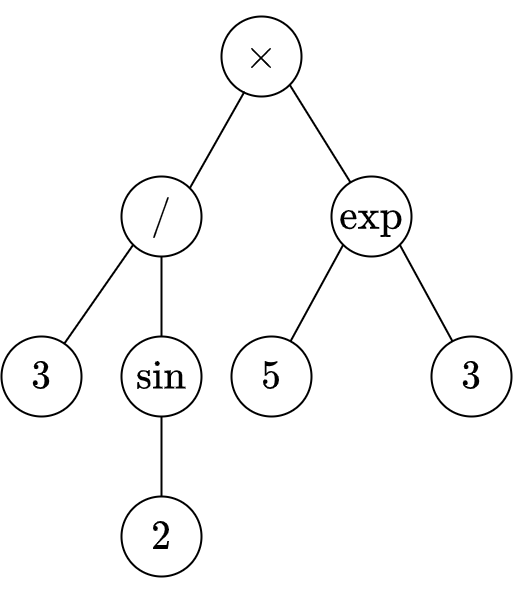
\includegraphics[height=5.5cm]{img/theoretical_framework/GP Initial Population 2.png}
      \caption{\(\mathbf{I}_2 = 7 - (5 + \sin(x))\)}
      \label{fig:genetic_programming:initialization:population:2}
    \end{subfigure}
    \begin{subfigure}[t]{0.4\textwidth}
      \centering
      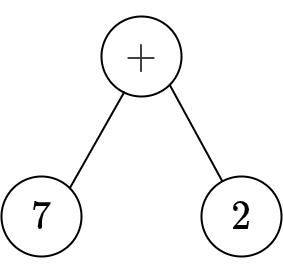
\includegraphics[height=2.75cm]{img/theoretical_framework/GP Initial Population 3.png}
      \caption{\(\mathbf{I}_3 = 7 + 2\)}
      \label{fig:genetic_programming:initialization:population:3}
    \end{subfigure}
    \begin{subfigure}[t]{0.4\textwidth}
      \centering
      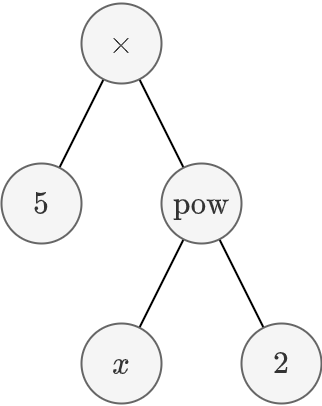
\includegraphics[height=4.125cm]{img/theoretical_framework/GP Initial Population 4.png}
      \caption{\(\mathbf{I}_4 = 5x^2\)}
      \label{fig:genetic_programming:initialization:population:4}
    \end{subfigure}
    \caption{A population of random trees.}
    \label{fig:genetic_programming:initialization:population}
  \end{figure}

  The next step is to calculate the fitness of each individual in the
  population.
  If we recall, the fitness function is the MSE between the expected output and
  the actual output of the individual.

  \begin{align*}
    \mathrm{MSE}(\mathbf{y}, \mathbf{I}_1[\mathbf{x}])
      & = \frac{1}{10} \sum_{i=1}^{10} (\mathbf{y}_i - \mathbf{I}_1(\mathbf{x}_i))^2
        = \frac{1}{10} \sum_{i=1}^{10} \left(
          \mathbf{y}_i - \frac{3}{\sin(2)} \cdot 5^3\right)^2 \\
      & \approx 177\,596.851\,131  \\
    \mathrm{MSE}(\mathbf{y}, \mathbf{I}_2[\mathbf{x}])
      & = \frac{1}{10} \sum_{i=1}^{10} (\mathbf{y}_i - \mathbf{I}_2(\mathbf{x}_i))^2
        = \frac{1}{10} \sum_{i=1}^{10} \left(
          \mathbf{y}_i - 7 - (5 + \sin(x_i))\right)^2 \\
      & \approx 137.398\,836  \\
    \mathrm{MSE}(\mathbf{y}, \mathbf{I}_3[\mathbf{x}])
      & = \frac{1}{10} \sum_{i=1}^{10} (\mathbf{y}_i - \mathbf{I}_3(\mathbf{x}_i))^2
        = \frac{1}{10} \sum_{i=1}^{10} \left(
          \mathbf{y}_i - (7 + 2)\right)^2 \\
      & \approx 331.924\,267 \\
    \mathrm{MSE}(\mathbf{y}, \mathbf{I}_4[\mathbf{x}])
      & = \frac{1}{10} \sum_{i=1}^{10} (\mathbf{y}_i - \mathbf{I}_4(\mathbf{x}_i))^2
        = \frac{1}{10} \sum_{i=1}^{10} \left(
          \mathbf{y}_i - 5x^2\right)^2 \\
      & \approx 138.079\,865
  \end{align*}

  With this, we can assign a fitness to each individual in the population as
  shown in \vref{tab:bg:gp:sym:init:pop}.
  A summary of the population's fitness is shown in
  \vref{tab:bg:gp:sym:init:pop:summary}.

  \subimport{.}{tab-bg-gp-sym-init-pop.tex}
  \subimport{.}{tab-bg-gp-sym-init-pop-summary.tex}

  We can observe that the worst individual has an error significantly larger
  than the best individual.
  This is to be expected, as the MSE is a measure of the error that escalates
  exponentially with the difference between the expected and actual output.  

  A graphical representation of the population is shown in
  \vref{fig:genetic_programming:initialization:population_graph}.
  It is clear from the figure that the worst individual is \(\mathbf{I}_1\).

  \begin{figure}[ht!]
    \centering
    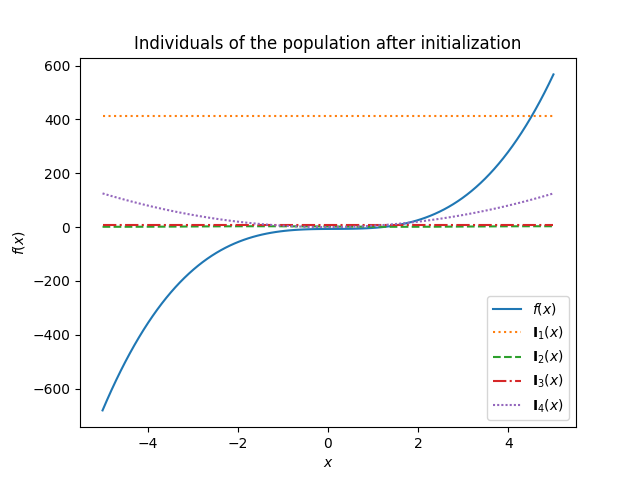
\includegraphics[width=0.6\textwidth]
      {img/theoretical_framework/gp_pop_init.png}
    \caption{
      Graphical representation of the population in generation 0 compared to the
      expected output.
    }
    \label{fig:genetic_programming:initialization:population_graph}
  \end{figure}

  In summary, the initialization phase plays a pivotal role in setting the 
  foundational landscape for the Genetic Programming process. Through randomized 
  generation methodologies, like the grow method, the algorithm nurtures a 
  diverse pool of candidate solutions. This diverse initial population enhances 
  the algorithm's probability of exploring different regions of the solution 
  space, thereby increasing the odds of locating an optimal solution. Yet, these 
  generated programs are merely starting points. Their evaluation, determined 
  through metrics such as the MSE, provides an empirical compass to guide the 
  evolution process. Once the fitness landscape has been charted out, the 
  algorithm is primed for the next pivotal phase: selection. In the upcoming 
  section, we delve into the mechanics of selection, a process crucial for 
  ensuring the survival and propagation of the fittest candidates.
